% =====================================================================
%  CUERPO DEL MANUAL DE CALIDAD - PharmaWeigh
% =====================================================================

\seccion{1. Acceso al sistema}

\tablaAcceso

\vspace{8pt}

Para ingresar al sistema:
\begin{enumerate}
    \item Abre tu navegador web (Chrome recomendado).
    \item Ve a la dirección \cd{https://pharma-formweigh.vercel.app}.
    \item Ingresa tu \campo{email} y tu \campo{contraseña}.
    \item Haz clic en \boton{Ingresar}.
\end{enumerate}

\begin{center}
\fbox{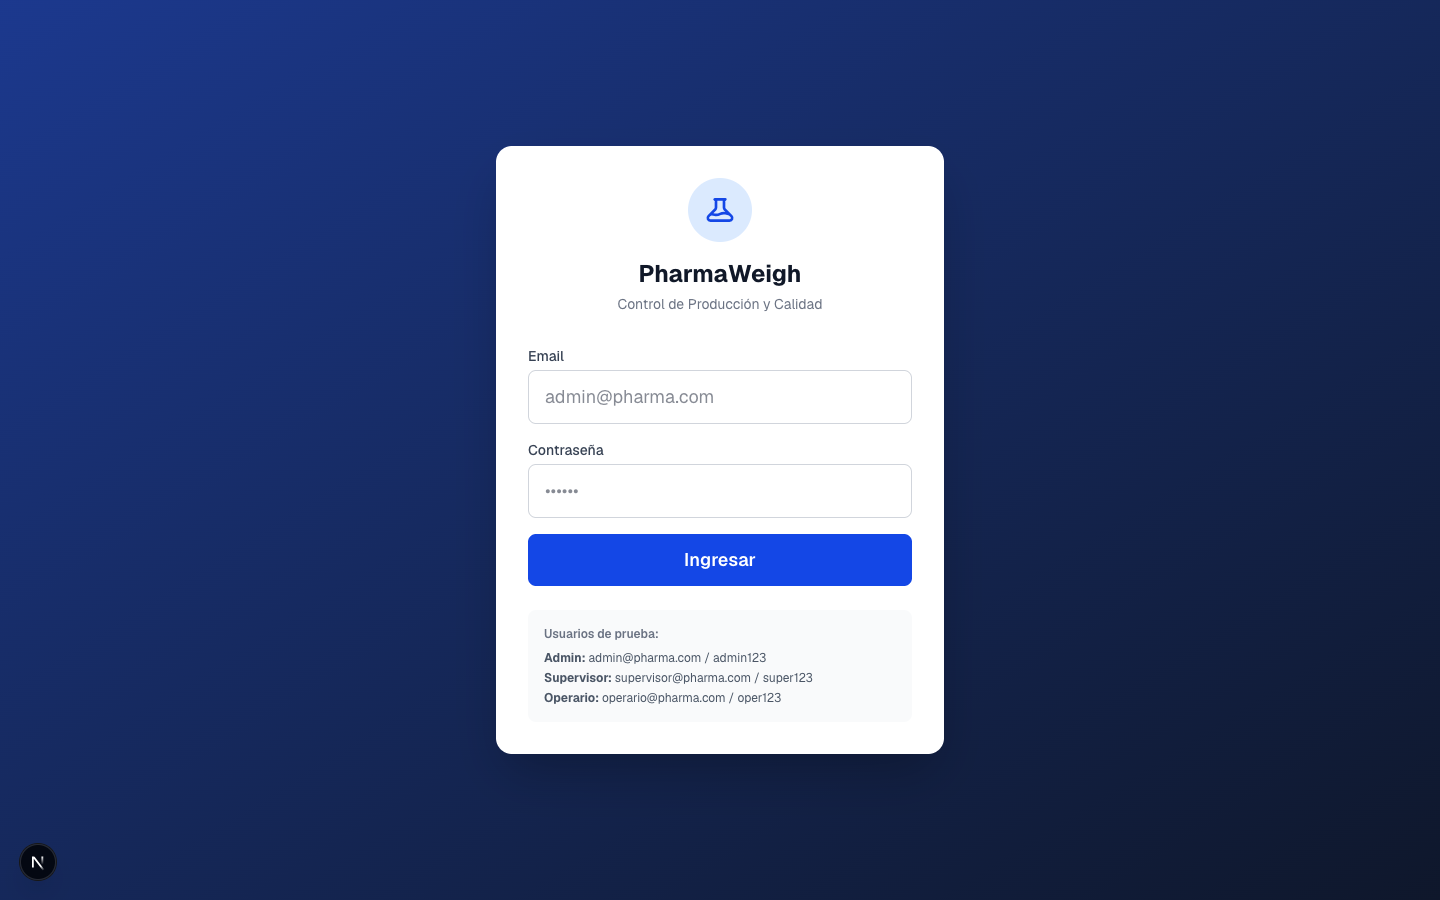
\includegraphics[width=0.85\linewidth]{capturas/01_login.png}}\\[3pt]
{\footnotesize\color{gristexto}Pantalla de inicio de sesión. Ingresa tu email y contraseña.}
\end{center}

Como analista de \textbf{Control de Calidad}, tu función es garantizar que los
materiales y procesos cumplan con las especificaciones y las Buenas Prácticas
de Manufactura (BPM/GMP).

\begin{cajaNota}
\textbf{Tu menú lateral muestra:} Dashboard, Órdenes (consulta), Dispensado (consulta),
Recetas (consulta), Inventario y Auditoría. No tienes acceso a Usuarios ni
Códigos de Barras.
\end{cajaNota}

% =====================================================================
\seccion{2. Tu rol en el proceso de producción}

Tu participación abarca \textbf{dos momentos clave}:

\vspace{6pt}
\begin{center}
\begin{tikzpicture}[
    node distance=0.3cm and 1.2cm,
    every node/.style={font=\footnotesize},
    paso/.style={draw=pharmablue, fill=pharmablue!8, rounded corners=6pt,
        minimum width=2.6cm, minimum height=1cm, align=center, text width=2.4cm},
    tuyo/.style={draw=pharmayellow, fill=pharmayellow!15, rounded corners=6pt,
        minimum width=2.6cm, minimum height=1cm, align=center, text width=2.4cm,
        line width=1.5pt},
    flecha/.style={-{Stealth[length=5pt]}, thick, color=gristexto}
]
\node[paso] (receta) {1. DESARROLLO\\Crear receta};
\node[tuyo] (lotes) {2. CALIDAD\\Aprobar lotes\\de materia prima};
\node[paso, right=of lotes] (super) {3. SUPERVISOR\\Crear orden};
\node[paso, below=1cm of receta] (oper) {4. OPERARIO\\Dispensar};
\node[tuyo, right=of oper] (firma) {5. CALIDAD\\Firmar y\\liberar lote};
\draw[flecha] (receta) -- (lotes);
\draw[flecha] (lotes) -- (super);
\draw[flecha] (super) |- (oper);
\draw[flecha] (oper) -- (firma);
\end{tikzpicture}
\end{center}
\vspace{6pt}

\begin{enumerate}
    \item \textbf{Antes de producción:} Apruebas o rechazas los lotes de materia prima.
    \item \textbf{Después del dispensado:} Firmas electrónicamente las fases completadas
          y liberas el lote de producto terminado.
\end{enumerate}

% =====================================================================
\newpage
\seccion{3. Dashboard}

\begin{center}
\fbox{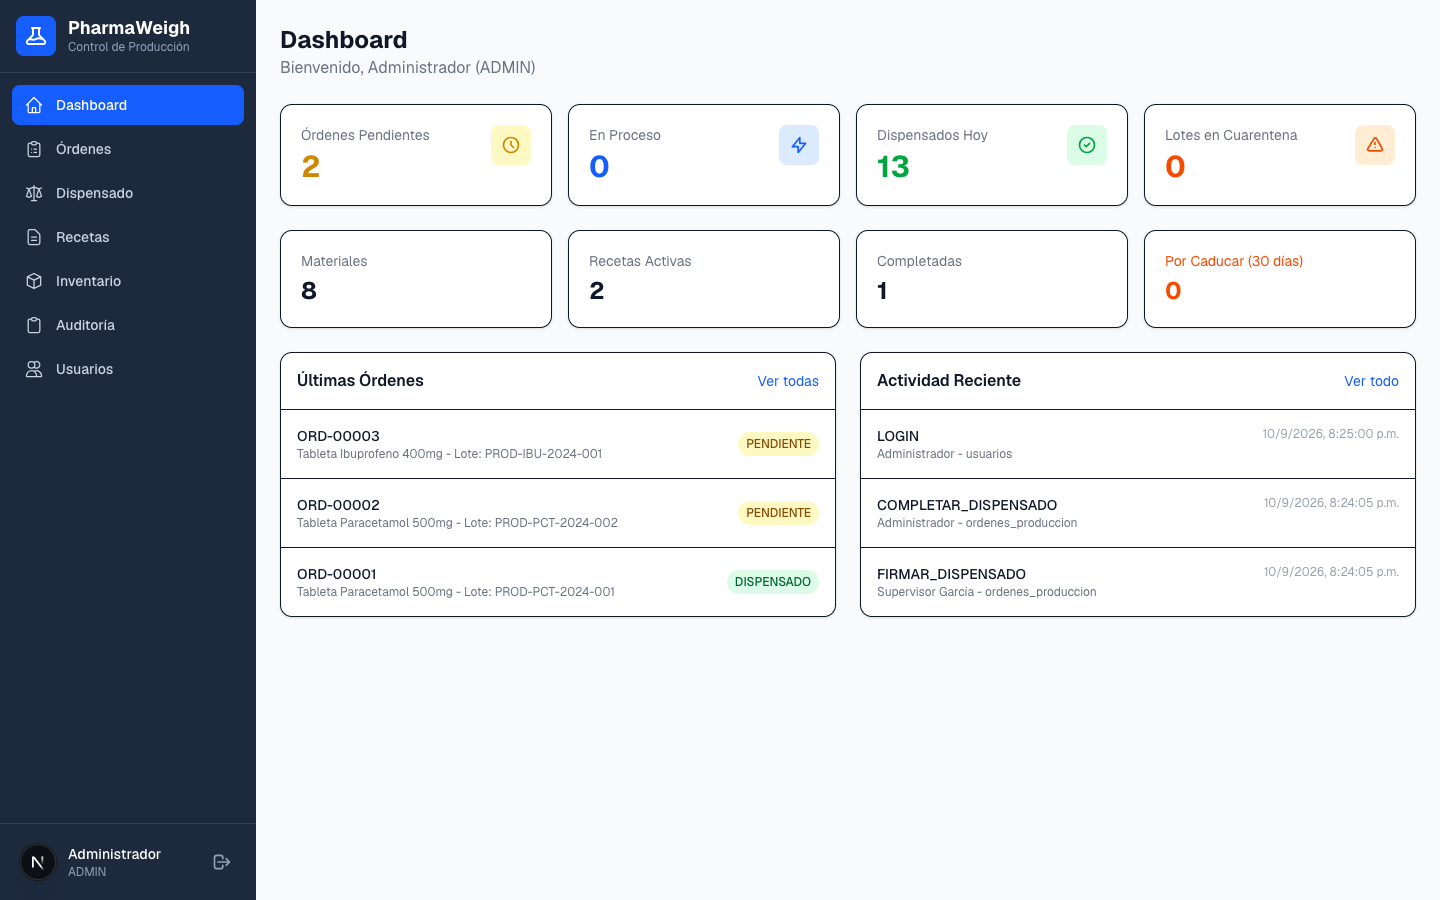
\includegraphics[width=0.92\linewidth]{capturas/03_dashboard.png}}\\[3pt]
{\footnotesize\color{gristexto}Dashboard principal con indicadores de producción.}
\end{center}

Como Calidad, los indicadores que más te interesan son:
\begin{itemize}
    \item \textbf{Lotes en Cuarentena} (naranja): lotes de materia prima pendientes
          de tu aprobación. \textbf{Este es tu indicador principal.}
    \item \textbf{Por Caducar (30 días)} (rojo): lotes próximos a vencer que
          requieren atención.
    \item \textbf{Dispensados Hoy} (verde): órdenes que podrían necesitar tu firma.
\end{itemize}

\begin{cajaTip}[Rutina diaria]
Al iniciar tu turno, revisa el dashboard. Si hay lotes en cuarentena,
apruébalos lo antes posible para no detener la producción. Si hay órdenes
dispensadas sin firmar, coordina con el supervisor.
\end{cajaTip}

% =====================================================================
\seccion{4. Aprobación y rechazo de lotes}

Esta es tu \textbf{responsabilidad principal}. Ningún lote puede usarse
en producción hasta que tú lo apruebes.

\subseccion{4.1 Flujo de estados de un lote}

\begin{center}
\begin{tikzpicture}[
    node distance=1.5cm,
    every node/.style={font=\small},
    estado/.style={draw, rounded corners=8pt, minimum width=2.5cm,
        minimum height=0.9cm, align=center, font=\small\bfseries},
    flecha/.style={-{Stealth[length=5pt]}, thick}
]
\node[estado, fill=pharmayellow!20, draw=pharmayellow] (cuarentena) {CUARENTENA};
\node[estado, fill=pharmagreen!20, draw=pharmagreen, right=of cuarentena] (aprobado) {APROBADO};
\node[estado, fill=pharmared!20, draw=pharmared, below=of cuarentena] (rechazado) {RECHAZADO};
\node[estado, fill=gray!20, draw=gray, below=of aprobado] (agotado) {AGOTADO};

\draw[flecha, color=pharmagreen] (cuarentena) -- node[above,font=\footnotesize\color{gristexto}]{Calidad aprueba} (aprobado);
\draw[flecha, color=pharmared] (cuarentena) -- node[left,font=\footnotesize\color{gristexto}]{Calidad rechaza} (rechazado);
\draw[flecha, color=gray] (aprobado) -- node[right,font=\footnotesize\color{gristexto}]{Se consume todo} (agotado);
\end{tikzpicture}
\end{center}

\subseccion{4.2 Aprobar o rechazar un lote paso a paso}

\begin{enumerate}
    \item Ve a \menu{Inventario} $\rightarrow$ pestaña \menu{Lotes}.
    \item Identifica los lotes con estado \cuarentena{} (badge amarillo).
    \item Para cada lote en cuarentena:
        \begin{itemize}
            \item Verifica el \textbf{certificado de análisis} del proveedor.
            \item Confirma que el material cumple con las especificaciones.
            \item Verifica la \textbf{fecha de caducidad}.
            \item Revisa las condiciones de almacenamiento.
        \end{itemize}
    \item Haz clic en \boton{Aprobar} si cumple, o \boton{Rechazar} si no cumple.
\end{enumerate}

\begin{center}
\fbox{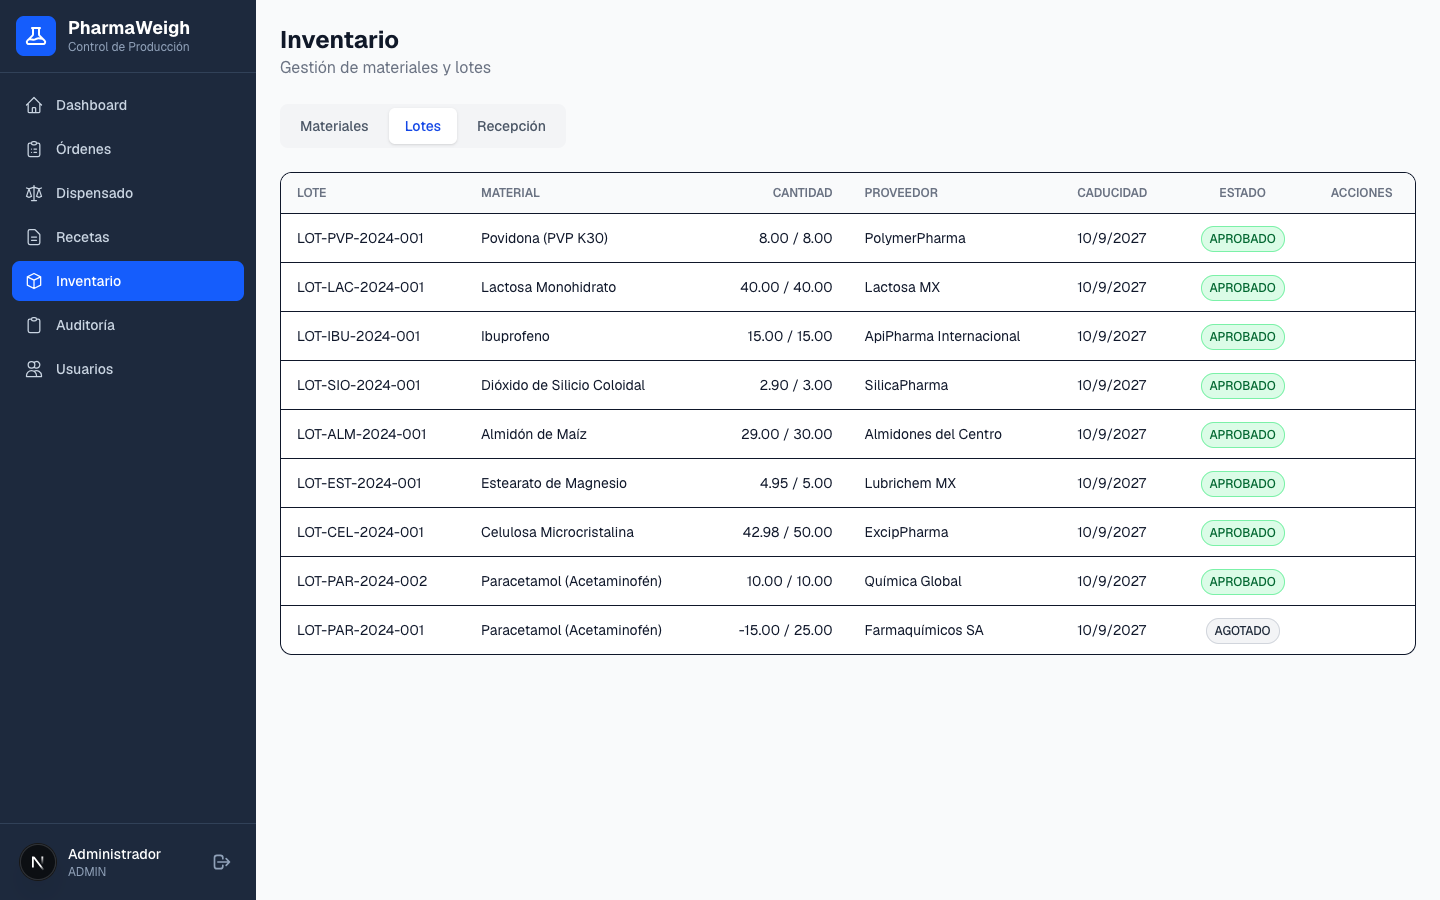
\includegraphics[width=0.92\linewidth]{capturas/15_inventario_lotes.png}}\\[3pt]
{\footnotesize\color{gristexto}Lista de lotes con estado. Los lotes en cuarentena tienen botones de Aprobar / Rechazar.}
\end{center}

\begin{cajaOjo}
\textbf{Un lote rechazado o en cuarentena NO puede usarse para dispensado.}
El sistema bloqueará cualquier intento de escanear un lote no aprobado.
Si rechazas un lote por error, puedes cambiar su estado de vuelta a cuarentena
y luego aprobarlo.
\end{cajaOjo}

\begin{cajaInfo}[Registro automático]
Cada cambio de estado se registra en la auditoría con tu nombre, fecha/hora,
estado anterior y nuevo. Este registro es \textbf{inmutable} y no puede borrarse.
\end{cajaInfo}

% =====================================================================
\newpage
\seccion{5. Firma electrónica de dispensados}

Después de que el operario termina de pesar todos los ingredientes de una fase,
el sistema solicita una \textbf{firma electrónica} de autorización.
Como Calidad, \textbf{puedes firmar dispensados}.

\subseccion{5.1 Proceso de firma}

\begin{enumerate}
    \item El operario o supervisor te llama a la estación de pesaje cuando aparece
          la pantalla de firma.
    \item \textbf{Verifica visualmente:}
        \begin{itemize}
            \item Que los contenedores correspondan a los materiales indicados.
            \item Que las etiquetas de lote sean legibles y correctas.
            \item Que el área de pesaje esté limpia.
        \end{itemize}
    \item Revisa el \textbf{Resumen de pasos} en pantalla: verifica que todos los
          pesos estén dentro de tolerancia (palomitas verdes).
    \item Ingresa tu \campo{email} (\cd{calidad@pharma.com}) y tu \campo{contraseña}.
    \item Haz clic en \boton{Firmar y Aprobar}.
\end{enumerate}

\begin{center}
\fbox{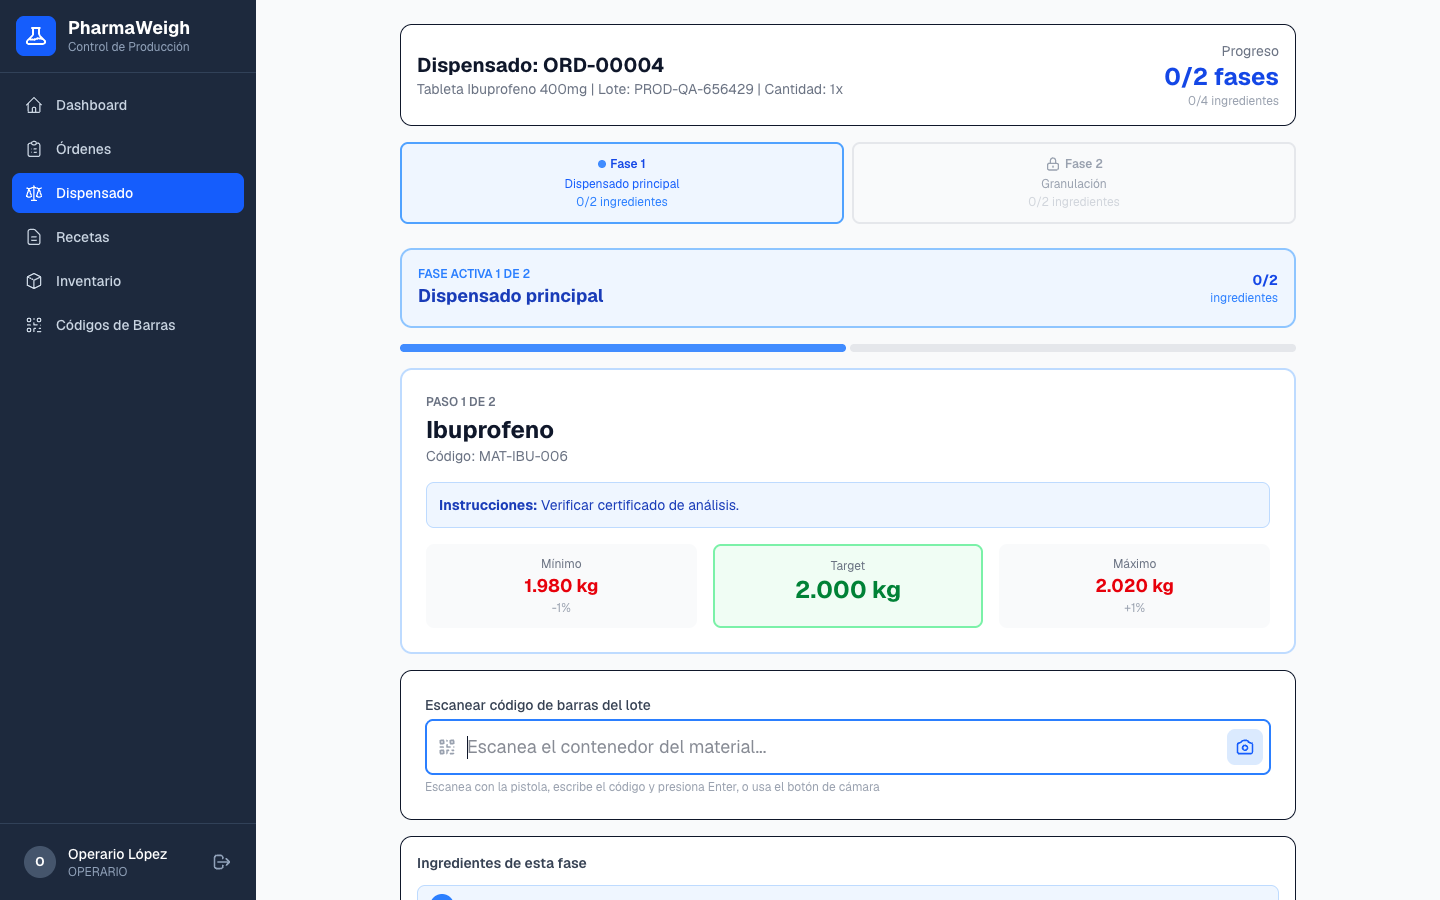
\includegraphics[width=0.92\linewidth]{capturas/06_dispensado_paso.png}}\\[3pt]
{\footnotesize\color{gristexto}Pantalla de dispensado con resumen de pasos e información del material actual.}
\end{center}

\begin{cajaOjo}
\textbf{Tu firma es legalmente vinculante (21 CFR Part 11).} Al firmar certificas que:
\begin{itemize}
    \item Los materiales dispensados son correctos.
    \item Los pesos están dentro de las tolerancias aprobadas.
    \item El proceso se ejecutó siguiendo las BPM.
\end{itemize}
\textbf{NO firmes sin verificar físicamente la estación.}
\end{cajaOjo}

\subseccion{5.2 ¿Quién puede firmar?}

\begin{center}
\begin{tabularx}{0.7\linewidth}{@{}l c@{}}
\toprule
\textbf{Rol} & \textbf{¿Puede firmar?} \\
\midrule
ADMIN      & Sí \\
SUPERVISOR & Sí \\
\textbf{CALIDAD}    & \textbf{Sí} \\
DESARROLLO & No \\
ALMACEN    & No \\
OPERARIO   & No \\
AUDITOR    & No \\
\bottomrule
\end{tabularx}
\end{center}

% =====================================================================
\newpage
\seccion{6. Auditoría y trazabilidad}

La auditoría es tu herramienta principal para verificar el cumplimiento.

\begin{center}
\fbox{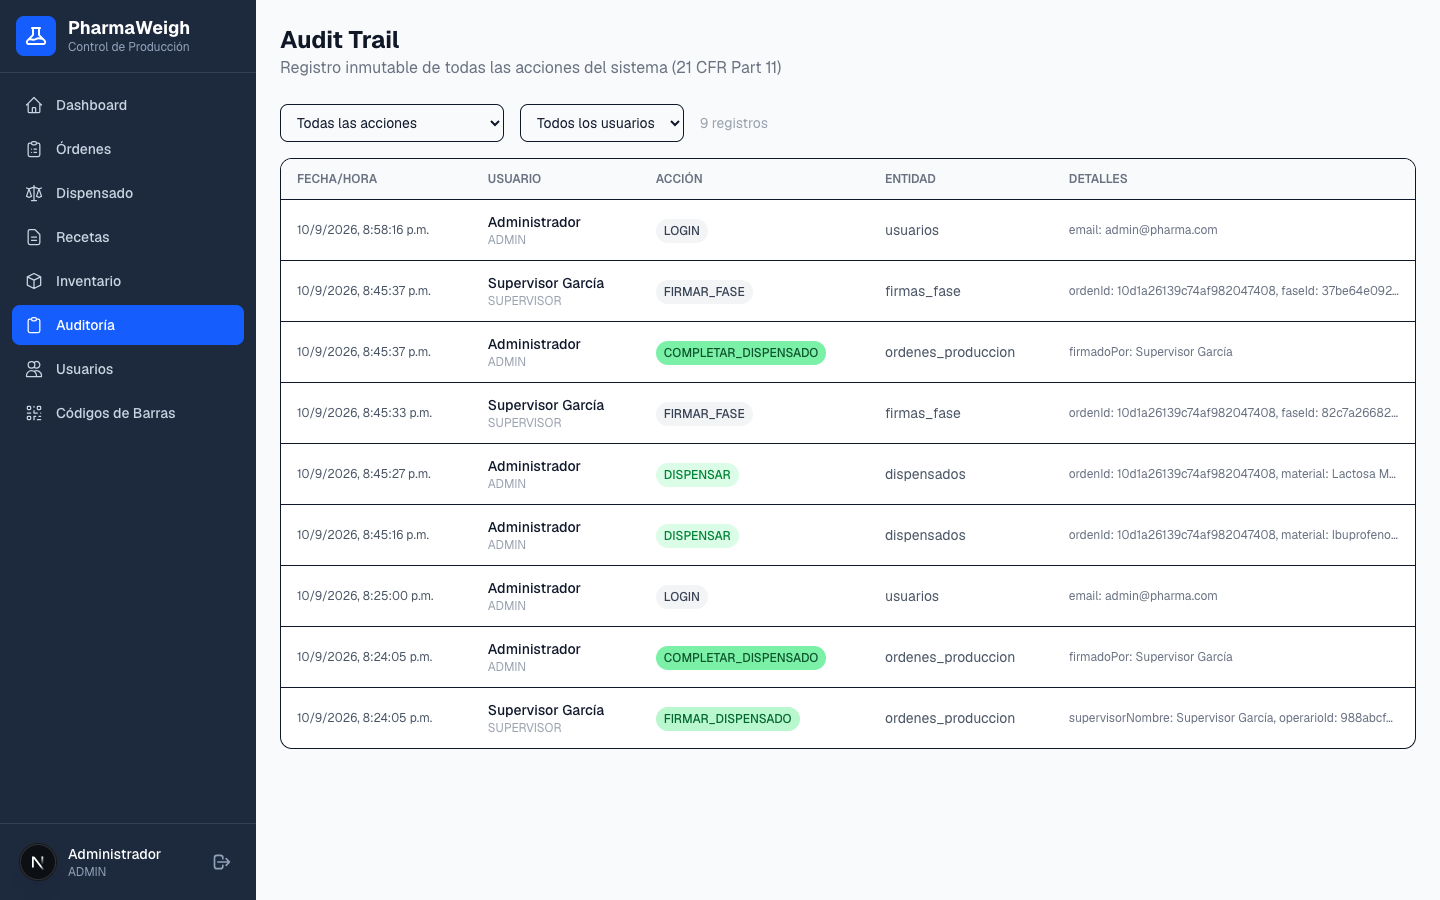
\includegraphics[width=0.92\linewidth]{capturas/17_auditoria.png}}\\[3pt]
{\footnotesize\color{gristexto}Log de auditoría: registro inmutable de todas las acciones del sistema.}
\end{center}

\subseccion{6.1 Consultas que debes hacer regularmente}

\begin{center}
\begin{tabularx}{\linewidth}{@{}l >{\raggedright\arraybackslash}X@{}}
\toprule
\textbf{Filtrar por} & \textbf{¿Qué verificas?} \\
\midrule
CAMBIAR\_ESTADO\_LOTE & Quién aprobó/rechazó cada lote y cuándo \\
DISPENSAR             & Peso real vs.\ target de cada material dispensado \\
FIRMAR\_FASE          & Quién firmó cada fase y en qué momento \\
COMPLETAR\_DISPENSADO & Órdenes terminadas y lista para tu revisión final \\
\bottomrule
\end{tabularx}
\end{center}

\subseccion{6.2 Cumplimiento 21 CFR Part 11}

El sistema cumple con los requisitos de la FDA para registros electrónicos:

\begin{center}
\begin{tabularx}{\linewidth}{@{}l >{\raggedright\arraybackslash}X@{}}
\toprule
\textbf{Requisito} & \textbf{Implementación} \\
\midrule
Registros electrónicos & Toda acción genera un registro inmutable con timestamp \\
Firmas electrónicas    & Email + contraseña, vinculante legalmente \\
Audit trail            & Log completo, no editable, no borrable \\
Control de acceso      & 7 roles con permisos diferenciados \\
Integridad de datos    & Base de datos con transacciones ACID \\
Trazabilidad           & Material $\rightarrow$ Lote $\rightarrow$ Orden $\rightarrow$ Operario $\rightarrow$ Firma \\
\bottomrule
\end{tabularx}
\end{center}

% =====================================================================
\newpage
\seccion{7. Equipo en la estación de pesaje}

Aunque no operas directamente el equipo, debes conocerlo para verificar
el proceso durante tus inspecciones.

\subseccion{7.1 Báscula de pesaje (ingreso manual)}

\begin{center}
\begin{tikzpicture}[
    every node/.style={font=\small}
]
\draw[fill=gray!10, draw=gray, rounded corners=4pt, line width=1pt]
    (0,0) rectangle (5,3);
\draw[fill=white, draw=gray!60, rounded corners=2pt]
    (0.5,1.5) rectangle (4.5,2.7);
\node[font=\Large\bfseries\color{pharmaazul}] at (2.5,2.1) {5.023 kg};
\node[font=\footnotesize\color{gristexto}] at (2.5,0.7) {Báscula analítica / de piso};

\draw[-{Stealth[length=6pt]}, thick, color=pharmablue] (5.3,1.5) -- (7,1.5)
    node[midway, above, font=\footnotesize\color{gristexto}] {El operario lee};
\node[draw=pharmablue, fill=pharmablue!5, rounded corners=4pt,
    minimum width=2.5cm, minimum height=1.5cm, align=center]
    at (8.5,1.5) {Ingresa el peso\\manualmente\\en PharmaWeigh};
\end{tikzpicture}
\end{center}

\begin{cajaNota}
La báscula \textbf{no está conectada} al sistema. El operario lee el peso
en la pantalla de la báscula y lo ingresa manualmente. El sistema valida
si el peso está dentro de la tolerancia definida en la receta.
\end{cajaNota}

\subseccion{7.2 Pistola láser (lector de código de barras)}

\begin{center}
\begin{tikzpicture}[
    every node/.style={font=\small}
]
\draw[fill=gray!15, draw=gray, rounded corners=3pt, line width=1pt]
    (0,0.5) -- (1.5,0.5) -- (2,1) -- (2,2.5) -- (1.5,3) -- (0,3) -- cycle;
\draw[fill=red!30, draw=red!60] (2,1.7) -- (3.5,1.2) -- (3.5,1.5) -- (2,2) -- cycle;
\node[font=\footnotesize\color{gristexto}] at (1,0) {Pistola láser USB};
\node[font=\tiny\color{red}] at (3.8,1.35) {Láser};

\draw[-{Stealth[length=6pt]}, thick, color=pharmablue] (4.2,1.5) -- (5.5,1.5);

\draw[fill=white, draw=gray, rounded corners=2pt]
    (5.8,0.3) rectangle (9.2,2.7);
\foreach \x in {6.1,6.3,6.4,6.7,6.8,7.1,7.2,7.4,7.7,7.8,8.0,8.2,8.4,8.6,8.8} {
    \draw[line width=1.2pt] (\x,0.8) -- (\x,2.2);
}
\node[font=\ttfamily\footnotesize] at (7.5,0.5) {LOT-PAR-2024-001};
\end{tikzpicture}
\end{center}

La pistola escanea el código de barras del lote. El sistema valida automáticamente
que sea el material correcto, esté aprobado, no esté caducado y tenga stock.

% =====================================================================
\newpage
\seccion{8. Preguntas frecuentes}

\subseccion{¿Puedo aprobar un lote que rechacé por error?}
No directamente. Pero puedes cambiar su estado de \rechazado{} a \cuarentena{}
y luego aprobarlo nuevamente. Ambas acciones quedan registradas en auditoría.

\subseccion{¿Qué pasa si no apruebo los lotes a tiempo?}
La producción se detiene. El operario no puede escanear lotes en cuarentena
ni rechazados. Aprueba los lotes lo antes posible para no generar cuellos
de botella.

\subseccion{¿Puedo ver quién dispensó cada material?}
Sí. En \menu{Auditoría} filtra por ``DISPENSAR''. Verás el operario,
material, peso real vs.\ target y si estuvo dentro de tolerancia.

\subseccion{¿Mi firma es diferente a la del supervisor?}
No. Ambas firmas tienen la misma validez legal. La diferencia es que como
Calidad tu enfoque es el \textbf{cumplimiento normativo}, mientras que el
supervisor se enfoca en la \textbf{operación}.

\subseccion{¿Qué verifico antes de firmar?}
\begin{enumerate}
    \item Todos los pasos tienen palomita verde (dentro de tolerancia).
    \item Los lotes usados corresponden a materiales aprobados.
    \item El área de pesaje está limpia y ordenada.
    \item Las etiquetas de los contenedores son legibles.
\end{enumerate}
